\documentclass{beamer}
\usepackage{multicol,lipsum,caption,graphicx}
\usepackage{mathtools, amsmath,booktabs,verbatim,tikz} 
\usetikzlibrary{shapes.geometric, arrows,positioning,matrix,calc}
%\usepackage{mathptmx}

\usetheme[progressbar=frametitle]{metropolis}
\setbeamertemplate{frame numbering}[fraction]
\useoutertheme{metropolis}
\useinnertheme{metropolis}
\usefonttheme{metropolis}
\usecolortheme{spruce}
\setbeamercolor{background canvas}{bg=white}

\title{Self-adaptative genetic algorithm for minimum thickness design of composite laminate}
\author{Huiyao Zhang}
\institute{Kyoto Institue of Technology}
\date{11-10-2020}
\setbeamertemplate{itemize/enumerate body begin}{\large}

\DeclarePairedDelimiter\Floor\lfloor\rfloor
\DeclarePairedDelimiter\Ceil\lceil\rceil
\begin{document}
\begin{frame}
    \titlepage
\end{frame}


\begin{frame}[c]{Content} 
    \begin{enumerate}
        \item Classic Lamination Theory
        \item Self-adaptative Genetic Algorithm
        \item Experiment and result
    \end{enumerate}
\end{frame}

\begin{frame}{1. Inspiration}
\begin{columns}[c]
    \begin{column}{0.9\textwidth}
        \begin{itemize}
			\item Paper: "Optimum design of composite laminates for minimum thickness"(Computers and
				Structures)
			\item Design Variable: Fiber orientation angles: [-90, 90], and layer thickness
			\item Search Method: Simulated annealing algorithm
			\item Constraint: safety factor $>$ 1
        \end{itemize}
    \end{column}
\end{columns}

\end{frame}

\begin{frame}{1. Problem with this work}
\begin{columns}[c]
    \begin{column}{0.4\textwidth}
        \begin{itemize}
			\item the search process wasn't presented
			\item the convergence speed, and the search cost
			\item GA is a better alternative
        \end{itemize}
    \end{column}

    \begin{column}{0.6\textwidth}
        \begin{center}
            \includegraphics[width=1.0\linewidth]{2020-11-10-pre-image/email.png}
        \end{center}
    \end{column}
\end{columns}


\end{frame}
\begin{frame}{2. Methdology}
    \begin{columns}[c]
    \begin{column}{1\textwidth}
		\begin{itemize}
			\item modifying selection strategy: in order to handle the constraint search
			\item Self-adaptative mutation direction of fiber orientation and laminate thickness:
				random change the length, and the angle in the laminate.
			\item the self-adaptative parameters don't refer to parent's proportion, mutation
				probability.
		\end{itemize}
    \end{column}
    \begin{column}{0.8\textwidth}

    \end{column}
\end{columns}
\end{frame}

\begin{frame}{2. Classic Lamination Theory}
    \begin{columns}[c]
    \begin{column}{0.5\textwidth}
		\begin{figure}
		\centering
		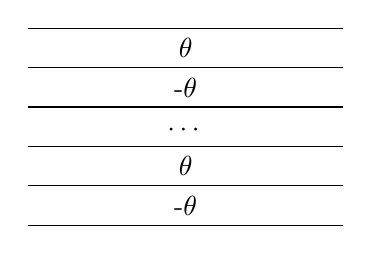
\begin{tikzpicture}
			\draw (0,0) -- (4,0);
			\draw (0,-0.5) -- (4,-0.5) node[midway, above] {$\theta$};
			\draw (0,-1) -- (4,-1) node[midway, above] {\text{-}$\theta$};
			\draw (0,-1.5) -- (4,-1.5) node[midway, above] {$\cdots$};
			\draw (0,-2) -- (4,-2) node[midway, above] {$\theta$};
			\draw (0,-2.5) -- (4,-2.5) node[midway, above] {\text{-}$\theta$};
		\end{tikzpicture}
		\caption{Model for Angle ply laminate}
		\end{figure}

        \includegraphics[width=0.8\linewidth]{GA_images/composite-material.png}
        \captionof{figure}{Composite Material}
    \end{column}
	\begin{column}{0.5\textwidth}
		\begin{equation} \label{eq:force_and_moments}
			\begin{array}{l}
				\begin{aligned}
			\begin{bmatrix}
				N_x \\
				N_y \\
				N_{xy}
			\end{bmatrix}
			&=
			\begin{bmatrix}
				A_{11} & A_{12} & A_{16} \\
				A_{12} & A_{22} & A_{26} \\
				A_{16} & A_{26} & A_{66} 
			\end{bmatrix}
			\begin{bmatrix}
				\varepsilon_x^0 \\
				\varepsilon_y^0 \\
				\gamma_{xy}^0
			\end{bmatrix}   \\
			&+               
			\begin{bmatrix}
				B_{11} & B_{12} & B_{16} \\
				B_{11} & B_{12} & B_{16} \\
				B_{16} & B_{26} & B_{66} 
			\end{bmatrix}
			\begin{bmatrix}
				k_x \\
				k_y \\
				k_{xy} 
			\end{bmatrix}  \\
		\end{aligned} \\ \\
		\begin{aligned}
			\begin{bmatrix}
				M_x \\
				M_y \\
				M_{xy}
			\end{bmatrix}
			&=
			\begin{bmatrix}
				B_{11} & B_{12} & B_{16} \\
				B_{12} & B_{22} & B_{26} \\
				B_{16} & B_{26} & B_{66} 
			\end{bmatrix}
			\begin{bmatrix}
				\varepsilon_x^0 \\
				\varepsilon_y^0 \\
				\gamma_{xy}^0
			\end{bmatrix} \\ 
			&+  
			\begin{bmatrix}
				D_{11} & D_{12} & D_{16} \\
				D_{11} & D_{12} & D_{16} \\
				D_{16} & D_{26} & D_{66} 
			\end{bmatrix}
			\begin{bmatrix}
				k_x \\
				k_y \\
				k_{xy} 
			\end{bmatrix}
		\end{aligned}
			\end{array}
		\end{equation}
	\end{column}
\end{columns}
\end{frame}

\begin{frame}{2. Self-adaptative GA: selection operator}
    \begin{columns}[c]
    \begin{column}{0.8\textwidth}
		\begin{itemize}
			\item acitve group: individual is used to increase the diversity of the population
			\item potential group: individual doesn't fulfill constraint
			\item proper group: individual meet constraint
		\end{itemize}
		
    \end{column}
\end{columns}
\end{frame}

\begin{frame}{2. Self-adaptative GA:  mutation operator}
    \begin{columns}[c]
    \begin{column}{1\textwidth}
		$\text{md} = [CT_1, \cdots, CT_{n-1}, CT_n] -  [ICV_0, \cdots, ICV_{n-1},
		ICV_n]$ \\
		\begin{itemize}
			\item  md means mutation direction.
			\item  $CT_i$ denotes the i-th constraint, such as weight, safety factor.
			\item  $ICV_i$ denotes individual's i-th constraint value, such as,  weight, safety
				factor of current individual.
		\end{itemize}

    \end{column}
\end{columns}
\end{frame}


\begin{frame}{2. Self-adaptative GA:  mutation operator}
    \begin{columns}[c]
	\begin{column}{1\textwidth}
		\begin{itemize}
			\item length mutation =  
				\[
				  \begin{cases}
					  LMC*[0, \sum_{i=1}^{N}{md_i}] & \text{if $\sum_{i=1}^{N}{md_i} > 0$} \\
					  LMC*[\sum_{i=1}^{N}{md_i}, 0] & \text{if $\sum_{i=1}^{N}{md_i} < 0$} \\
				  \end{cases}
				\] \\
				LMC stands for length mutation coefficient, it's a positive integer.
			\item angle mutation = 
				\[
				  \begin{cases}
					  AMC*[0, \sum_{i=1}^{N}{md_i}] & \text{if $\sum_{i=1}^{N}{md_i} > 0$} \\
					  AMC*[\sum_{i=1}^{N}{md_i}, 0] & \text{if $\sum_{i=1}^{N}{md_i} < 0$} \\
				  \end{cases}
				\] \\
				AMC stands for angle mutation coefficient, it's sign is unclear.
		\end{itemize}
	\end{column}
\end{columns}
\end{frame}



\begin{frame}{Result: Loading $N_x = 10, N_y=5 $ MPa m}
    \begin{columns}
    \begin{column}{0.5\textwidth}

        \begin{center}
            \includegraphics[width=1.0\linewidth]{2020-11-10-pre-image/two_distinct_angle_fitness_and_sr.png}
        \end{center}

        \begin{center}
              \includegraphics[width=1.0\linewidth]{2020-11-10-pre-image/two_distinct_angle_angle_change.png}
        \end{center}
    \end{column}
    \begin{column}{0.5\textwidth}
        \begin{center}
              \includegraphics[width=1.0\linewidth]{2020-11-10-pre-image/two_distinct_angler_number_change.png}
              \captionof{figure}{Two distinct angles in the laminate}
        \end{center}
    \end{column}
\end{columns}
\end{frame}


\begin{frame}{Result: Loading $N_x = 10, N_y=5 $ MPa m}

\begin{table}
	\normalsize
\caption{Comparison with the results of DSA}
\label{tab:comparision}
\centering
	\resizebox{10cm}{!}{
\begin{tabular}{c|cccc|lccc}
	\toprule
	\textbf{Loading}	    & \multicolumn {4}{c}{\textbf{Akbulut and Sonmez's\cite{akbulut2008optimum} Study}}   & \multicolumn {4}{c}{\textbf{Present Study}}\\
	\midrule
	 $N_{x}/N_{y}/N_{xy}$   & Optimum lay-up			        & laminate  & TW & MS   & Optimum lay-up & laminate  & TW & MS \\
	  (MPa m)	            & sequences					        & thickness &    &      & sequences	     & thickness &    &    \\
	\midrule
	  10/5/0                 &  $[37_{27}/\text{-}37_{27}]_s$     &  108      &  1.0068  &  1.0277 & $[33_{29}/\text{-}39_{25}/\bar{\text{-}39}]_s$     &     109      &  1.0074      &  1.0246  \\
	  20/5/0                 &  $[31_{23}/\text{-}31_{23}]_s$     &  92       &  1.0208  &  1.1985 & $[33_{22}/\text{-}31_{24}]_s$                      &     92      &  1.0055       &  1.2065    \\
	  40/5/0                 &  $[26_{20}/\text{-}26_{20}]_s$     &  80       &  1.0190  &  1.5381 & $[29_{18}/\text{-}21_{23}/\bar{\text{-}21}]_s$     &     83      &  1.0034       &  1.7350   \\
	  80/5/0                 &  $[21_{25}/\text{-}19_{28}]_s$     &  106      &  1.0113  &  1.2213 & $[\text{-}20_{27}/21_{25}/\bar{25}]_s$             &     105      &  1.0029      &  1.2063    \\
	  120/5/0                &  $[17_{35}/\text{-}17_{35}]_s$     &  140      &  1.0030  &  1.0950 & $[\text{-}18_{34}/17_{36}]_s$                     &     140      &  1.0000      &  1.0898     \\
	\bottomrule
\end{tabular}
}
\end{table}
\end{frame}



\end{document}
